\section{UPPAAL SMC}\label{sec:smc}
UPPAAL \gls{smc} is one of the newer versions of UPPAAL, it works with statistical model checking for more efficient analysis, as it avoids the exhaustive exploration of the state-space. This statistical exploration gives the added benefit of significantly less memory consumption, meaning that the computers physical memory is rarely the limit when running a query. This flexibility allows for \gls{smc} to be used in other areas which was previous too memory intensive for other UPPAAL tools\cite{cs_smc}. \\
As mentioned in \myref{sec:upp_cora}, \gls{cora} only support linear rates, \gls{smc} facilitates non-linear rates and differential equations, which makes it possible to implement \gls{kibam}, based on our information from \myref{sec:kibam} this will greatly improve our battery estimations. \gls{smc} looks similar to previous tools in UPPAAL in form of GUI, but it adds new functionality which will be showcased in the rest of this section, this will include probability and simulate queries and how the results of these queries can be interpreted and understood. \\
Lets say we want to check what the probability for the system reaching a specific location. First we model the system as shown in \cref{fig:example}, which contains one initial and four other locations. The initial locations is committed, which means that time is not allowed to pass when we are in that location.

\begin{figure}[H]
	\centering
	\begin{tikzpicture}
	%Locations
	\node [init] (l0) {C};
	\node [location] (l1) [right of=l0, xshift=10mm,yshift=10mm, label={
		[align=left]above right:
		\textcolor{name}{L1}
	}] {};
	\node [location] (l2) [right of=l0, xshift=10mm, yshift=-10mm, label={
		[align=left]below right:
		\textcolor{name}{L2}
	}] {};
	\node [location] (l3) [left of=l0, xshift=-10mm, yshift=-10mm, label={
		[align=left]below left:
		\textcolor{name}{L3}
	}] {};
	\node [location] (l4) [left of=l0, xshift=-10mm, yshift=10mm, label={
		[align=left]above left:
		\textcolor{name}{L4}
	}] {};
	%Edges
	\path[->,black, thick] (l0) edge (l1);
	\path[->,black, thick] (l0) edge (l2);
	\path[->,black, thick] (l0) edge (l3);
	\path[->,black, thick] (l0) edge (l4);
	\end{tikzpicture}
	\caption{Model for showcasing probability}
	\label{fig:example}
\end{figure}

\begin{equation}\label{eq:q1}
Pr[<=1](<> Process.L4)
\end{equation}

With this system we are now able to ask if the system reach a specified location by the query shown in \cref{eq:q1}. Pr is a keyword to denote that we want to find the probability, square brackets describe the amount of time to pass, it is possible to specify which clock to use, by adding the variable name of the clock at the beginning in between the square brackets. \\
Alternative you can swap out time for discrete steps by putting hash(\#) in the same place as clock variables. In the parentheses we want to check if we reach location \uppLoc{L4}, Process refers to the model also known as a template, and the diamond (<>) describe that a path can reach location \uppLoc{L4}, another option is to use square bracket ([]) which mean that a property must be true during the entire path. In this example is dose not make sense because in this example we want to see if we can reach location \uppLoc{L4}. \\
Running the query in \cref{eq:q1} return the following probability range [0.18744,0.287382] that roughly translate to 18.7\%-28.7\% which is based on (294 runs), this result has a 95\% certainty because the probability uncertainty($\epsilon$) is default set to 0.05 (5\%), along with two other interesting parameters, probability of false negatives($\alpha$) and probability of false positive($\beta$). In \cref{table:smc_result} the results from running the query in \cref{eq:q1} with different parameter setting can be seen. The first row shows that running query with $\alpha$ = 0.05, $\beta$ = 0.05 and $\epsilon$ = 0.05 results in a 18.7\%~ to 28.7\%~ probability of reaching \uppLoc{L4}. Likewise the time it took to finish the query was 9 milliseconds. The rest of the row shows the effect of change the parameter of those setting, the $\alpha$ and $\beta$ are exclusive used in hypothesis testing by \gls{smc}  and by the table they have a profound effect on the probability range when used in conjunction with probability uncertain. This can be seen in row 5 which uses both a lower $\alpha$, $\beta$ and $\epsilon$, resulting only in a range from 23.5-28.5\%~ probability.

\begin{table}[]
	\centering
	\scalebox{0.8}{
	\begin{tabular}{|l|l|l|l|l|l|}
		\hline
		\multicolumn{3}{|c|}{Results} & \multicolumn{3}{c|}{Parameters} \\ \hline
		Runs & Execution time & Probability & $\alpha$ & $\beta$ & $\epsilon$ \\ \hline
		294 & 0.009s & {[}0.18744,0.287382{]} & 0.05 & 0.05 & 0.05 \\ \hline
		1107 & 0.062s & {[}0.199776,0.249758{]} & 0.05 & 0.05 & 0.025 \\ \hline
		271 & 0.017s & {[}0.160035,0.25979{]} & 0.05 & 0.025 & 0.05 \\ \hline
		370 & 0.026s & {[}0.179833,0.279827{]} & 0.025 & 0.05 & 0.05 \\ \hline
		1585 & 0.072s & {[}0.235516,0.285492{]} & 0.025 & 0.025 & 0.025 \\ \hline
	\end{tabular}}
	\caption{Results from Pr[<=1](<> Process.L4) with different parameter settings}
	\label{table:smc_result}
\end{table}

Simulate was another feature introduced in \gls{smc}, it is used to run the modelled system a number of time and capture some values during simulation, to illustrate this a new model it needed, which can be found in \cref{fig:showcase01} along with its declarations in \cref{lst:showcase1_declarations}. Three clock are defined in this example, and a model that has two locations where it is possible to go from one location to the other when the clock t is between $[5-10]$. Depending on the location either \uppVar{x} or \uppVar{y} can increment with respectively rates 1 and 2.

\begin{figure}[H]
	\begin{lstlisting}[language=my_c, caption={Declarations}, label=lst:showcase1_declarations]
	clock x, y, t;
	\end{lstlisting}
\end{figure}

\begin{figure}[H]
	\centering
	\begin{tikzpicture}
	%Locations
	\node [init] (l0) [label={
		[align=left]left:
		\textcolor{invariant}{x '== 1}\\
		\textcolor{invariant}{\&\& y '== 0}\\
		\textcolor{invariant}{\&\& t <= 10}
	}] {};
	\node [location] (l1) [right of=l0, xshift=20mm, label={
		[align=left]right:
		\textcolor{invariant}{x '== 0}\\
		\textcolor{invariant}{\&\& y '== 2}\\
		\textcolor{invariant}{\&\& t <= 10}
	}] {};
	%Edges
	\path[->,black, thick] (l0) edge[bend left=30] node [midway, above][align=left]{
			\textcolor{guard}{t >= 5}\\
			\textcolor{update}{t = 0}
		} (l1);
	\path[->,black, thick] (l1) edge[bend left=30] node [midway, below][align=left]{
			\textcolor{guard}{t >= 5}\\
			\textcolor{update}{t = 0}
		} (l0);
	\end{tikzpicture}
	\caption{Simple model}
	\label{fig:showcase01}
\end{figure}

Simulations can now be done with the newly modelled system, the queries for these can be seen in \cref{eq:q2}, in these simulation it runs 100time units, and the values specified to be captured during the simulations is \uppVar{x} and \uppVar{y}.

\begin{equation}\label{eq:q2}
simulate 1 [<= 100] {x,y}
simulate 5 [<= 100] {x,y}
\end{equation}

\begin{figure}[!h]
	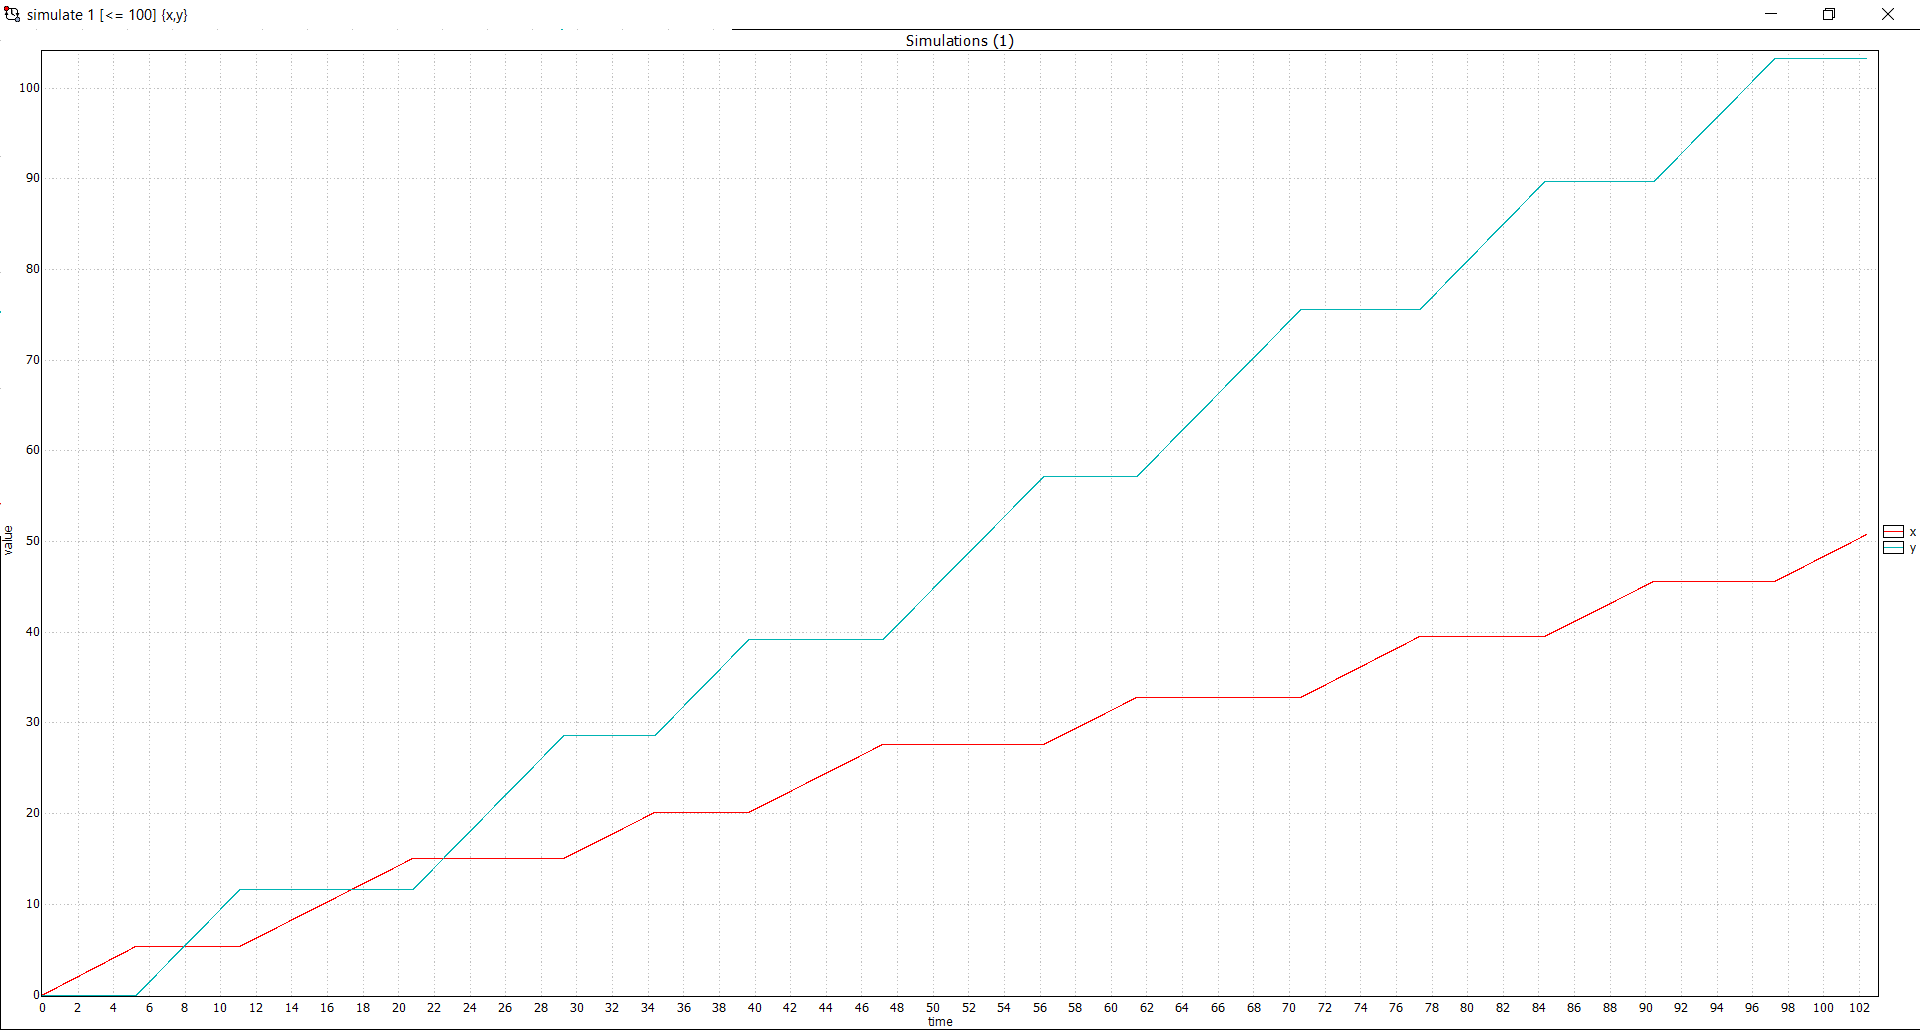
\includegraphics[width=\textwidth]{graphics/showcase01.png}
	\caption{One simulations of the value of two variables \uppVar{x, y} over 100time units}
	\label{fig:sim01}
\end{figure}

\begin{figure}[!h]
	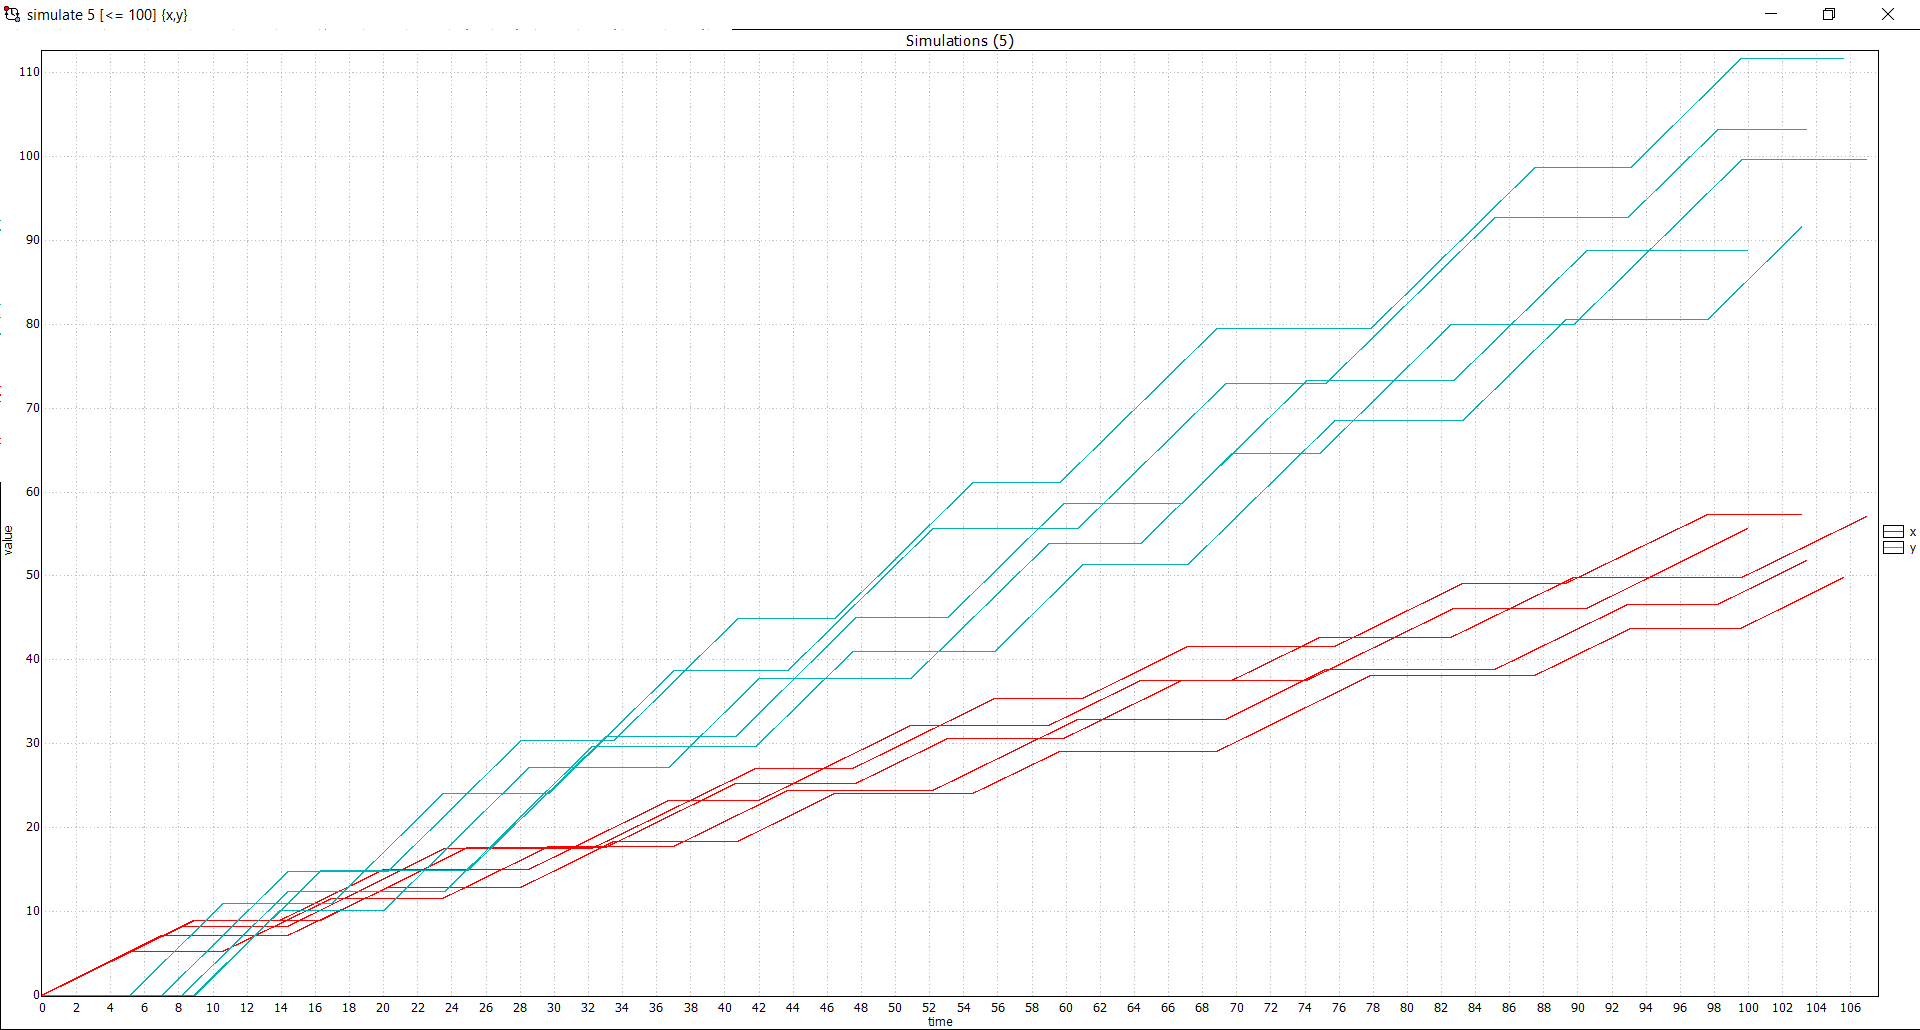
\includegraphics[width=\textwidth]{graphics/showcase02.png}
	\caption{Five simulations of the value of two variables \uppVar{x, y} over 100time units}
	\label{fig:sim02}
\end{figure}

Two graphs shows the data gather during simulation, in \cref{fig:sim01} and \cref{fig:sim02}. Where the y axis is value and x is time. The simulation runs the system random, if randomness is modelled in the system and will therefore generate new values for the graph each time it is run. Examining the graph we can observe that the value \uppVar{x} tends to around 50 within 100time units, so a new question can be raised \textit{``What is the probability that x is above or equal to 50 when 100time units have passed?''} in \cref{eq:q3} a query have been constructed to answer the question.

\begin{equation}\label{eq:q3}
Pr[<=150](<> x >= 50)
\end{equation}

Like the previous probability example, the query gives us a range of what the probability is that x will be higher or equal to 50 when 100 time units have passed, which in this query results in having a 98\%~ to 100\%~ probability. It is possible to get more information from the query in the form of seven different graphs (probability density distribution, Probability Density Confidence Intervals, Probability Distribution, Probability Confidence Intervals, Cumulative Probability Distribution, Cumulative Probability Confidence Intervals, and Frequency Histogram). 

Frequency Histogram shows the count on the y axis and run duration in time on the x axis, each of the columns represent a time where a number of runs have fulfilled the property. So the first column show that out of the 263 runs three of them had observed the value \uppVar{x} to be higher or equal to 50 at 80.8time units. This histogram show that with a 99\% certainty \uppVar{x} will at the earliest be 50 or higher at 80.8 and latest 111.4time units.

\begin{figure}[!h]
	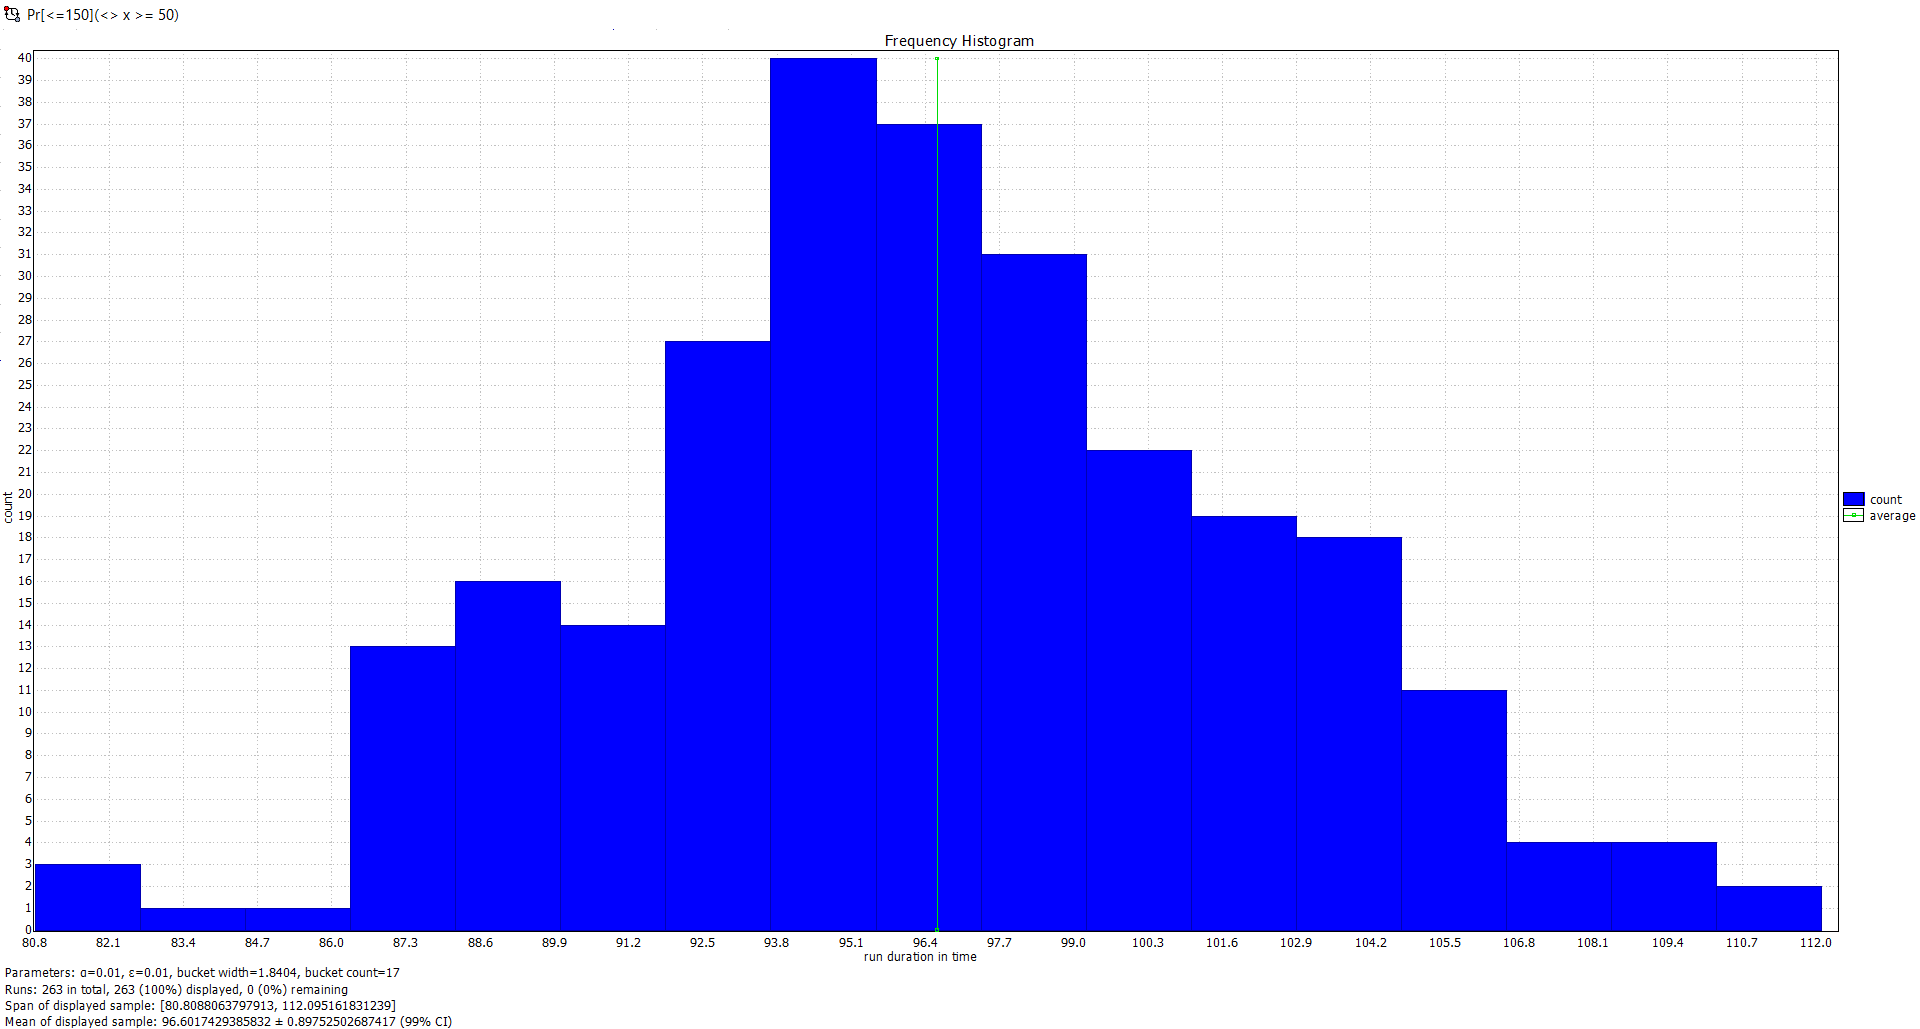
\includegraphics[width=\textwidth]{graphics/eq3fh.png}
	\caption{Frequency histogram generated from \cref{eq:q3}}
	\label{fig:eq3fh}
\end{figure}

Cumulative Probability Distribution shows the accumulated probability over time, so with a 99\% certainty at 112time units it has a 100\% probability for \uppVar{x} to be equal or above 50, and at 96.4time units there is a 50\% probability.

\begin{figure}[!h]
	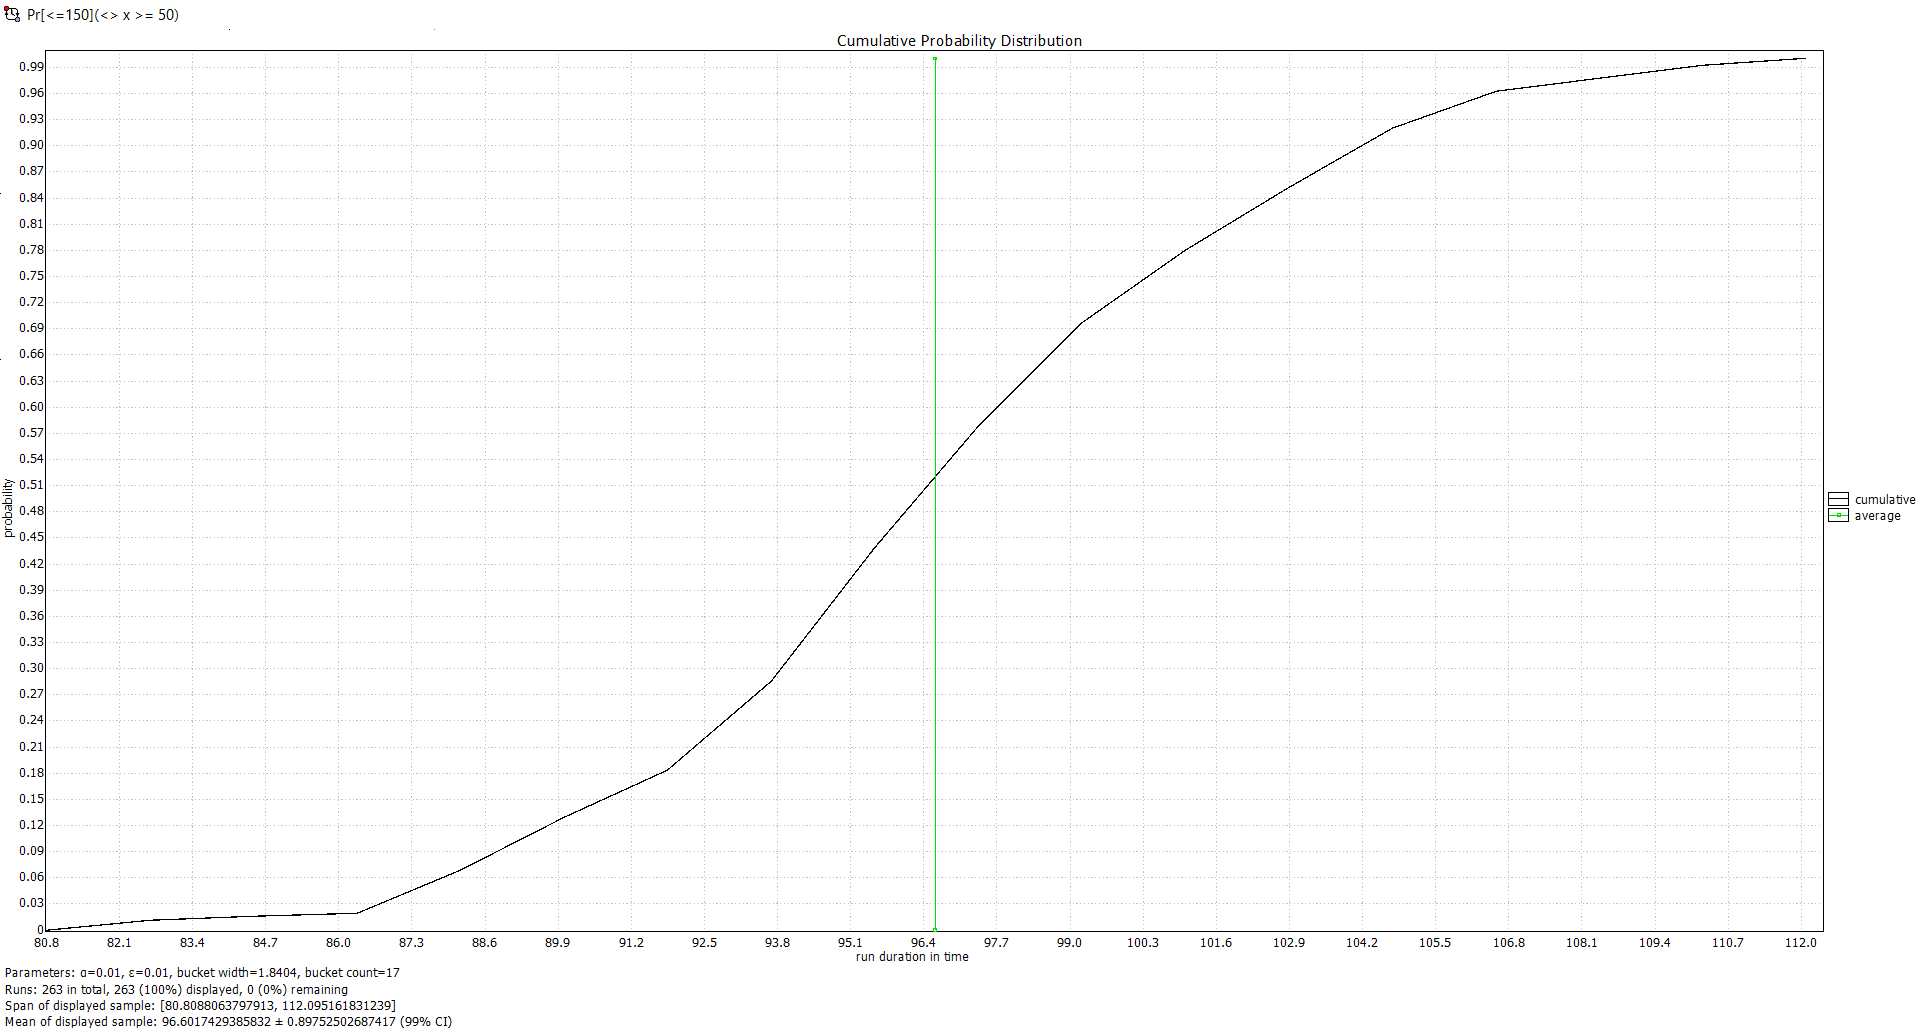
\includegraphics[width=\textwidth]{graphics/eq3cpd.png}
	\caption{Cumulative probability distribution generated from \cref{eq:q3}}
	\label{fig:eq3cpd}
\end{figure}

The graphs generated by SMC from queries can give useful information about the probability for a query and even more insight, an example of this can be seen the above graphs, when running the query it only returns the probability, but by looking at the graphs we are able to also extract that if this system run for 112 or more time units \uppVar{x} will always be 50 or higher.

%TODO describe queries and afterwards the results.


